\chapter{Framework }\label{ch:work}
\section{JPEG AI Verification Model}\label{sec:vm}
%tipi dei dati, struttura, target bpp e altri parametri.
Lo strumento utilizzato per l'estrazione delle feature è \textit{jpeg-ai-reference-software} \cite{jpeg-ai-ref-sw}; questo rappresenta l'implementazione del sistema proposto nominato \textit{JPEG AI Verification Model}. Sono messi a disposizione due encoder: \texttt{Enc0}, il più semplice, implementabile su dispositivi mobili, ed \texttt{Enc1}, più complesso, composto da \textit{attention blocks} e\textit{ transformer}, che richiedono una capacità di computazione elevata.
\\Sono supportati tre diversi "operation point" \textit{SOP, BOP, HOP}, forniti rispettivamente per dispositivi dotati di CPU, dispositivi mobili, e dispositivi dotati di hardware specializzato come le GPU.\\
Interessante è la feature chiamata \textit{Multi-branch Decoding} \ref{fig:multibranch}, per la quale sono presenti tre diverse \textit{synthesys transform} \ref{sec:architetturaJPEGAI} per ogni \textit{operation point}: il bitstream può essere decodificato da una qualsiasi di queste tre, lasciando così la libertà al dispositivo di scegliere quale livello di complessità è più adatto per le proprie capacità computazional; anche un'immagine compressa con l'encoder più complesso, può essere decodificata da un decoder più semplice. 
\begin{figure}
    \centering
    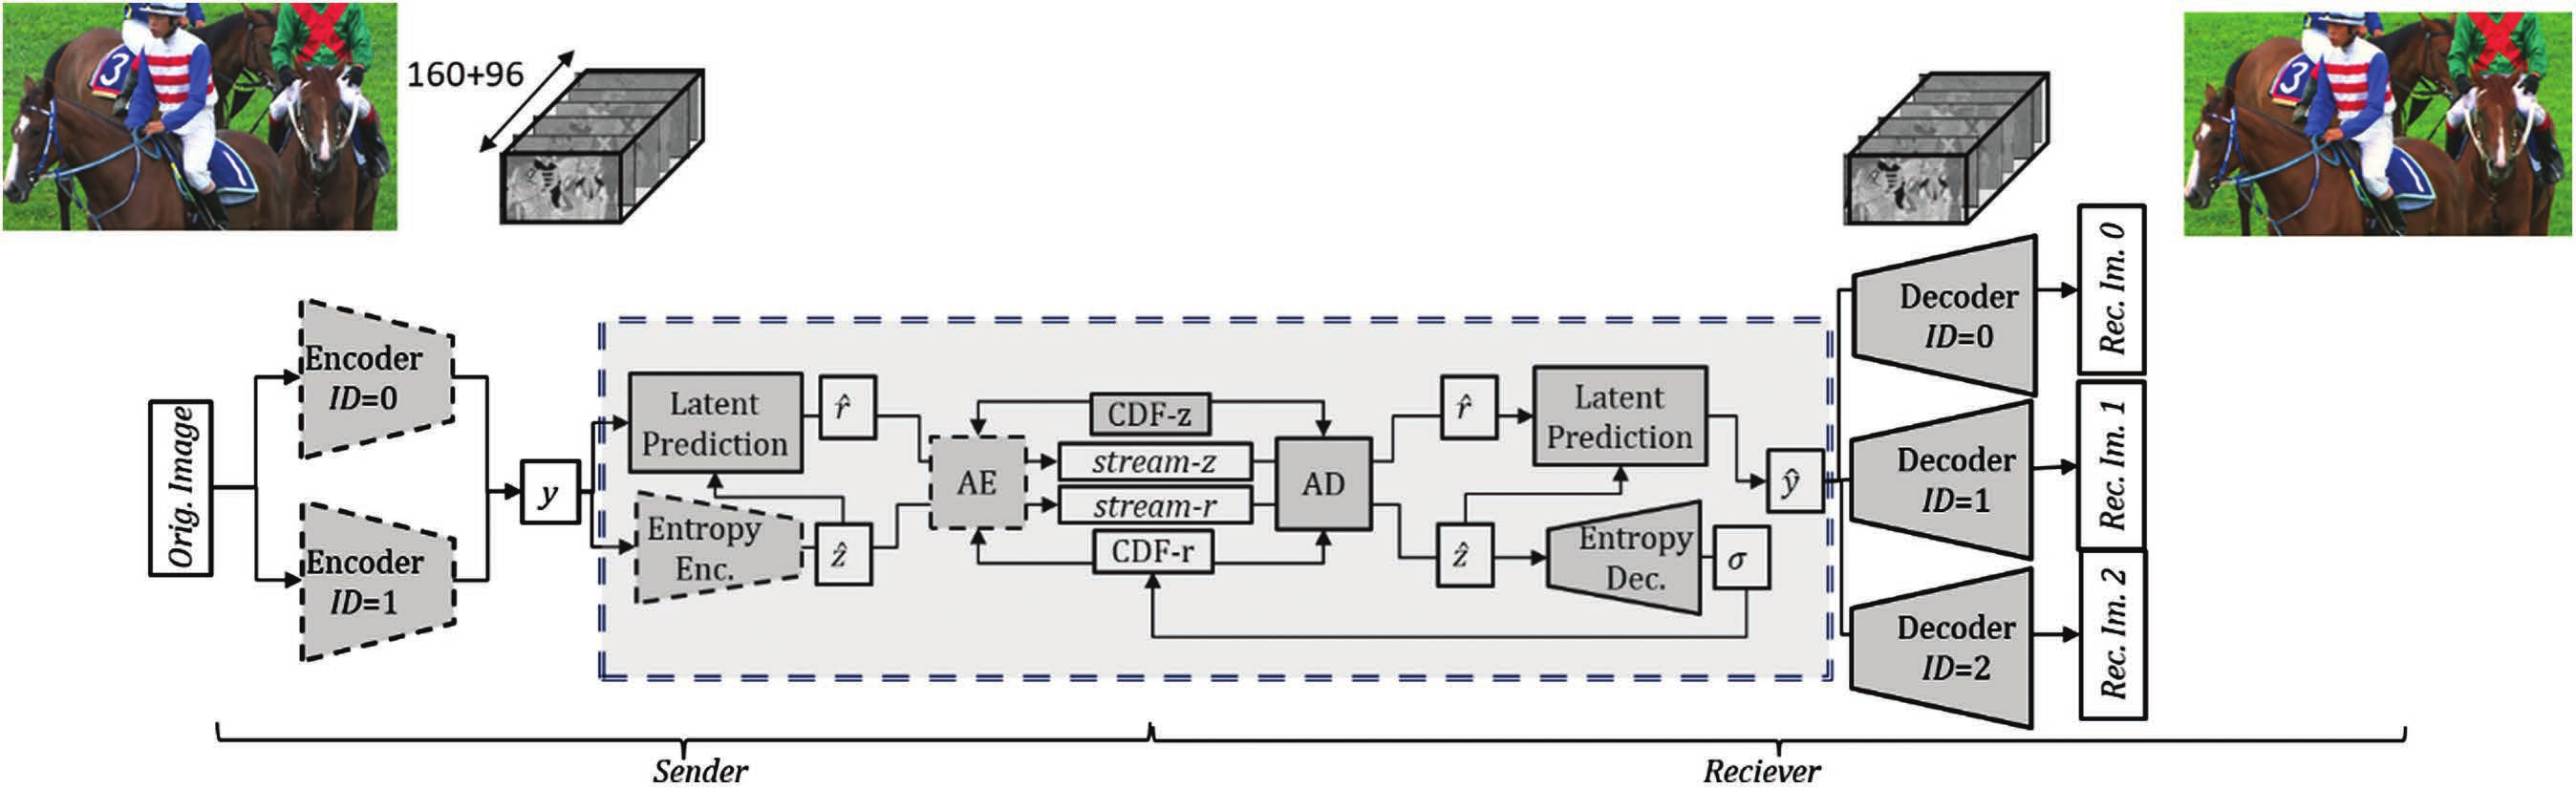
\includegraphics[width=1\linewidth]{img/multi-branch.png}
    \caption{Multi-branch decoding}
    \label{fig:multibranch}
\end{figure}
\paragraph{Rappresentazioni estratte} Le immagini prima di essere elaborate dall'encoder vengono pre-processate: inizialmente convertite nel formato YUV BT.709, separando le componenti di luminanza e crominanza, e successivamente viene applicato quello che è chiamato \textit{Conditional Color Separation}, un approccio per cui il componente primario, la luminanza (Y), viene compresso con una rete neurale più potente, mentre la crominanza viene compressa usando informazioni della luminanza \cite{ccs}; così si abbassa il picco dell'utilizzo della memoria, permettendo una riduzione nella complessità computazionale .\\
La separazione delle componenti è mantenuta anche nel bitstream finale \ref{fig:bitstream}, dando la possibilità di scartare la parte di crominanza se non necessaria per alcune applicazioni.
\begin{figure}
    \centering
    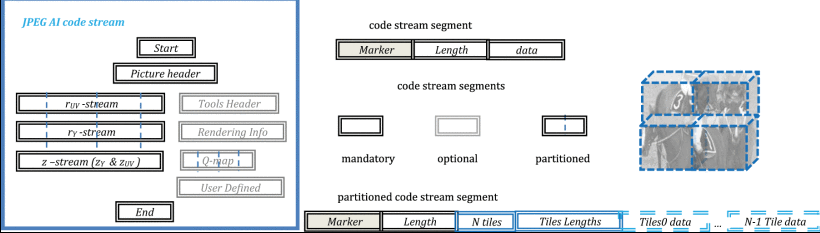
\includegraphics[width=1\linewidth]{img/JPEG AI codestream.png}
    \caption{JPEG AI bitstream}
    \label{fig:bitstream}
\end{figure}
\section{Random Forest e GridSearchCV}
%framework usato, perche scelti questi modelli,
Come framework per la parte di machine learning è stata usata \textit{Scikit-learn}, una libreria open-source scritta in Python, considerata come una delle più importanti per il \textit{machine-learning}.\\
Come classificatori è stato scelto RandomForest, ...\\ \textit{spiegazione teorica di RandomForest e GridSearch???}
\subsection{Addestramento}
I modelli sono stati addestrati direttamente sulle rappresentazioni latenti prodotti dall'encoder di JPEG AI, in particolare alcuni su $y$ e altri su $\hat{y}$ (vedi fig. \ref{fig:architmin}) per avere un confronto tra i due
\begin{itemize}
    \item $y$ rappresenta l'output dell'\textit{Analysis transform} (vedi fig.\ref{fig:encodingJPEGAI})
    \item $\hat{y}$ rappresenta l'input dell'\textit{Synthesis transform} (vedi fig. \ref{fig:decodingJPEGAI})
\end{itemize}
L'encoder genera dei tensori separati per la luminanza e la crominanza, rispettivamente con 160 e 96 canali.
\textit{parlare del numero di immagini usate}
\section{Dataset utilizzato}\label{sec:dataset}
Il dataset usato negli esperimenti è \textit{140k Real and Fake Faces} \cite{140kRealFake}, una raccolta di 140.000 immagini di volti, suddivise in 70.000  immagini reali e 70.000 immagini fake.\\
Le immagini reali fanno parte del dataset \textit{Flickr-Faces-HQ} (FFHQ) \cite{NVlabsFfhqdataset2025}, e consistono in fotografie di volti umani in alta qualità distinte da altri dataset per la presenza di una grande varietà di soggetti per età ed etnia, ma anche per la presenza di accessori come occhiali o cappelli \cite{karras2019style}; queste immagini sono state collezionate da Flickr, un servizio web che offre la possibilità di pubblicare immagini ad artisti e fotografi.
Le immagini fake invece fanno parte del dataset \textit{1 Milion Fake Faces} ,un insieme di immagini generate tramite StyleGAN (vedi sez. \ref{par:style}.
\paragraph{Suddivisione dati} I dati sono già suddivisi in training set, test set, e validation set, rispettivamente composti da 100000, 20000 e 20000 immagini; ogni insieme mantiene un perfetto bilanciamento tra le due classi. Il perfetto bilanciamento lo rende ideale per l'addestramento, e la suddivisione nei vari set semplifica molto la preparazione dei dati.
%\subsection{StyleGAN}\label{sec:style}
%\cite{karras2019style}
